\documentclass{article}
\usepackage[margin=1in]{geometry}
\usepackage[utf8]{inputenc}
\usepackage{graphicx} 
\usepackage{fancyhdr}
\usepackage{enumitem}
\usepackage{lipsum}
\usepackage[bahasa]{babel}
\usepackage{subcaption}
\usepackage{float}
\usepackage{indentfirst}
\usepackage{hyperref}

\title{Laporan Workshop Telematika \\ ESP8266 Minimum System} % Ganti sesuai modul praktikum yang diikuti
\author{Ikhwanul Abiyu Dhiyya'ul Haq \\ 5024211048} % Ganti dengan NRP dan Nama Kalian

\date{}


\fancypagestyle{firstpageheader}{
  \fancyhf{} 
  \fancyhead[L]{
\includegraphics[height=1.5cm]{img/logodepart.png}} 
  \fancyhead[R]{Institut Teknologi Sepuluh Nopember \\ Departemen Teknik Komputer \\ Laboratorium Robotika dan Sistem Cerdas} 
  \renewcommand{\headrulewidth}{0pt} 
  \fancyfoot[C]{%
    
\includegraphics[width=\textwidth]{img/footer.png}
  }
  \renewcommand{\footrulewidth}{0pt} % No line in the footer
}


\fancyhf{} 
\fancyfoot[C]{%
  
\includegraphics[width=\textwidth]{img/footer.png}
}
\renewcommand{\headrulewidth}{0pt} 
\renewcommand{\footrulewidth}{0pt} 

\pagestyle{fancy}
\begin{document}
\selectlanguage{bahasa}
\maketitle
\thispagestyle{firstpageheader}
% Bagian Tugas Pendahuluan
\section*{Tugas Pendahuluan}
\begin{enumerate}
  \item Jelaskan bagaimana cara kontrol 7-segment anoda dan katoda? \\
  Jawaban : 
  
  7-segment anoda dikontrol dengan cara memberikan tegangan logika 1 pada pin yang terhubung dengan anoda, sedangkan 7-segment katoda dikontrol dengan cara memberikan tegangan logika 0 pada pin yang terhubung dengan katoda.

  \item Buat schematic untuk menampilkan nomor kelompok menggunakan dua 7-segment! \\
  Jawaban : 
  
  Terlampir

\end{enumerate}

\newpage
% Bagian Analisis Hasil Percobaan
\section*{Analisis Hasil Percobaan}
\indent
% Pada gambar \ref{fig:inirujukan} dapat dilihat bahwa pada tabel \ref{tab:labelini}

Pada praktikum ke-1 tentang Desain PCB menggunakan Fusion 360, kami membuat sebuah desain PCB dari rangkaian \textit{minimal system} ESP8266, rangkaian ini terdiri dari ESP8266, Connector UART, Connector Power, Regulator 3.3V (SOT223), 5 Resistor, 2 Kapasitor, dan 2 Switch. Rangkaian \textit{minimal system} dapat dilihat pada gambar \ref{fig:rawcircuit}.

\begin{figure}[htbp]
    \centering
    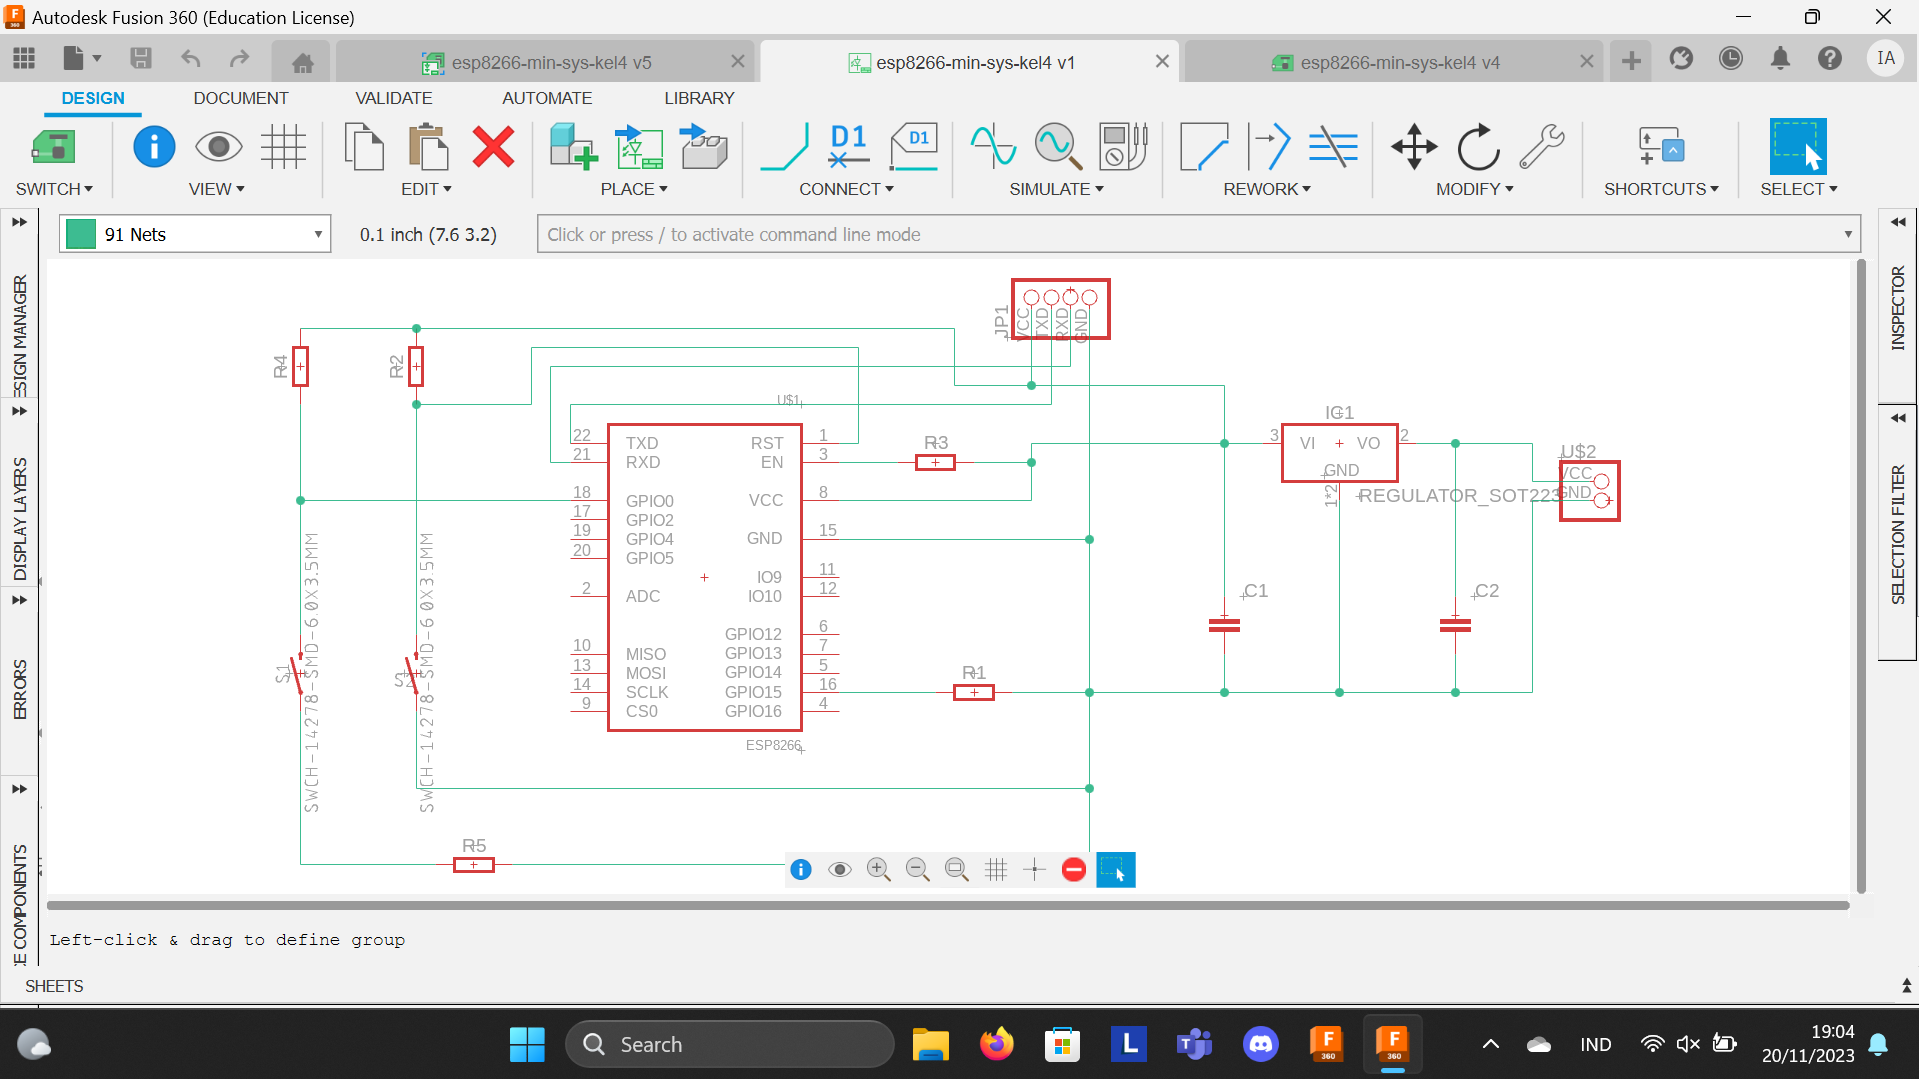
\includegraphics[width=0.4\textwidth]{img/raw-circuit.png}
    \caption{Desain Circuit \textit{Minimal System} ESP8266}
    \label{fig:rawcircuit}
\end{figure}

Setelah itu, kami mendesain layout PCB dari rangkaian \textit{minimal system} ESP8266 tersebut. Layout PCB dapat dilihat pada gambar \ref{fig:pcb-assembled}.

\begin{figure}[htbp]
    \centering
    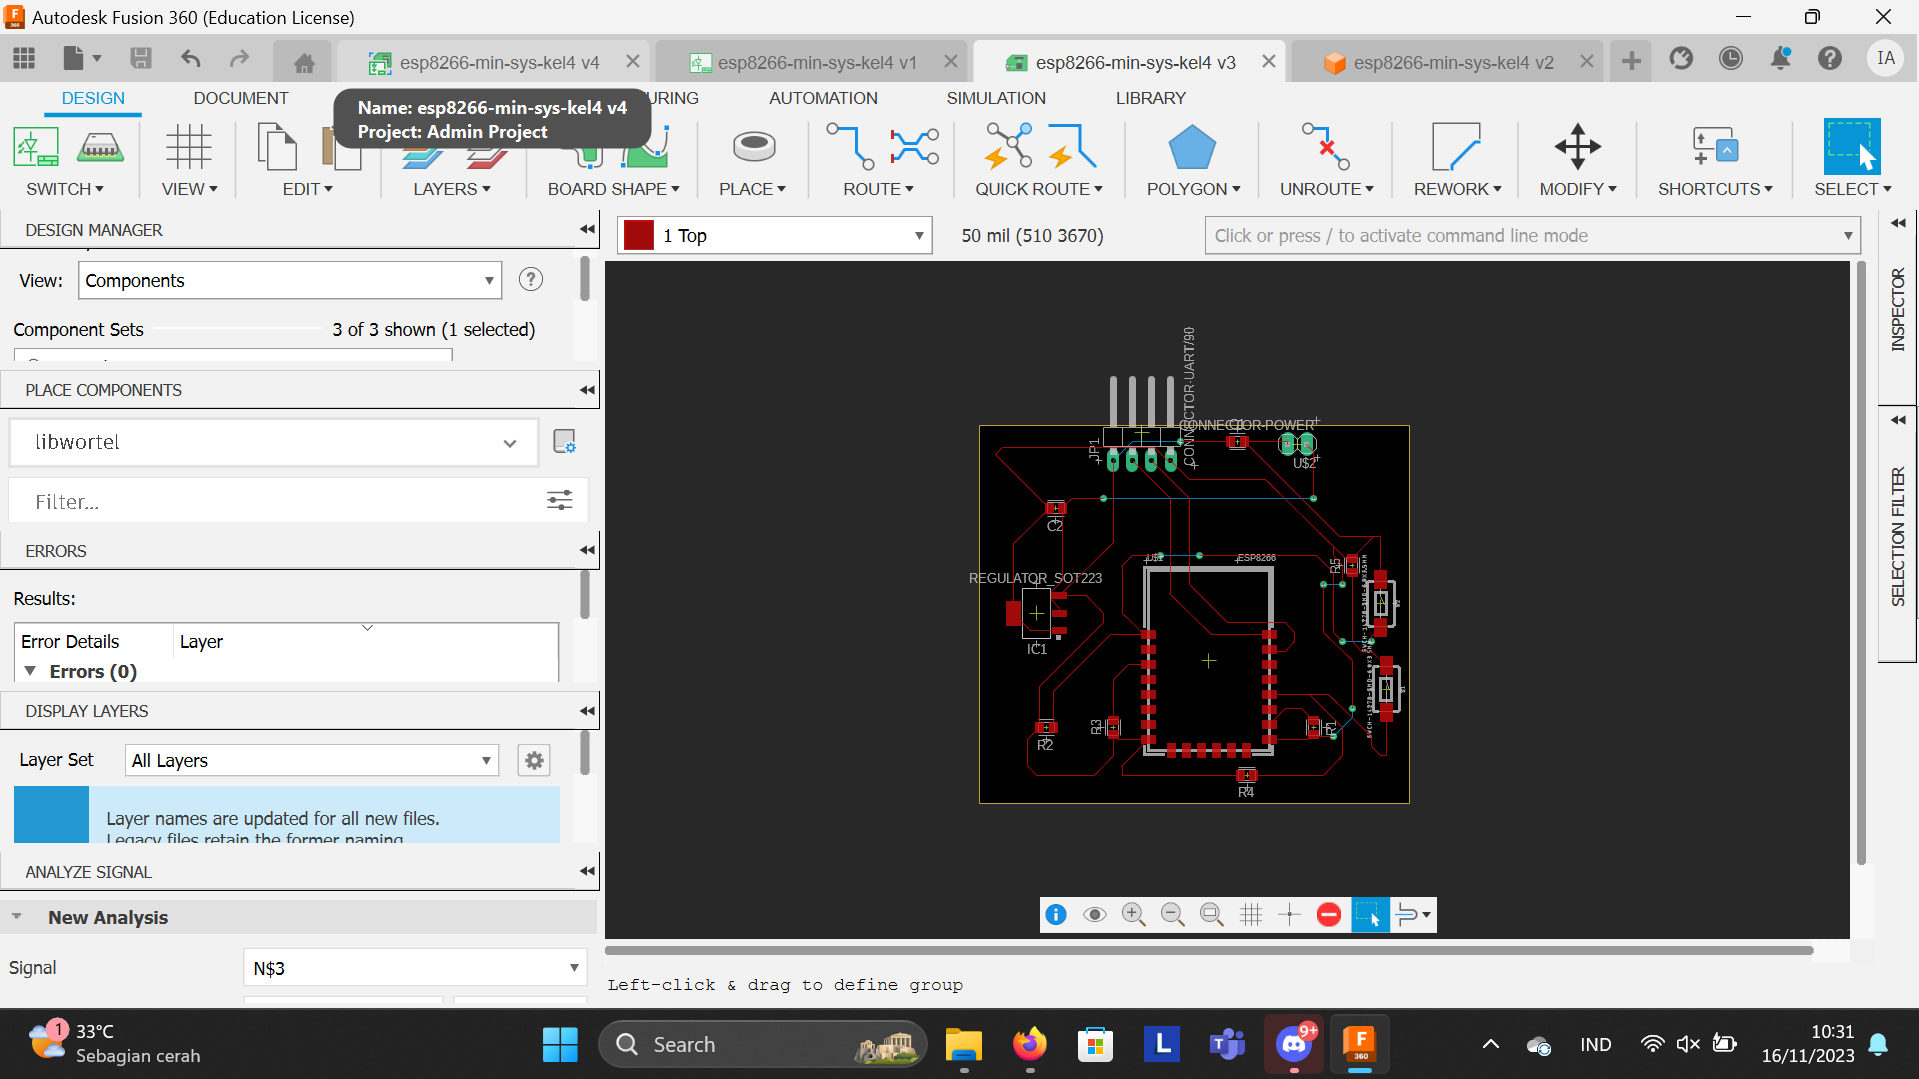
\includegraphics[width=0.4\textwidth]{img/pcb-assembled.png}
    \caption{Desain PCB yang telah dibuat \textit{layout}-nya}
    \label{fig:pcb-assembled}
\end{figure}

Setelah itu, kami men-\textit{generate} 3D model dari PCB yang telah dibuat. 3D model dapat dilihat pada gambar \ref{fig:3dmodel}.

\begin{figure}[htbp]
    \centering
    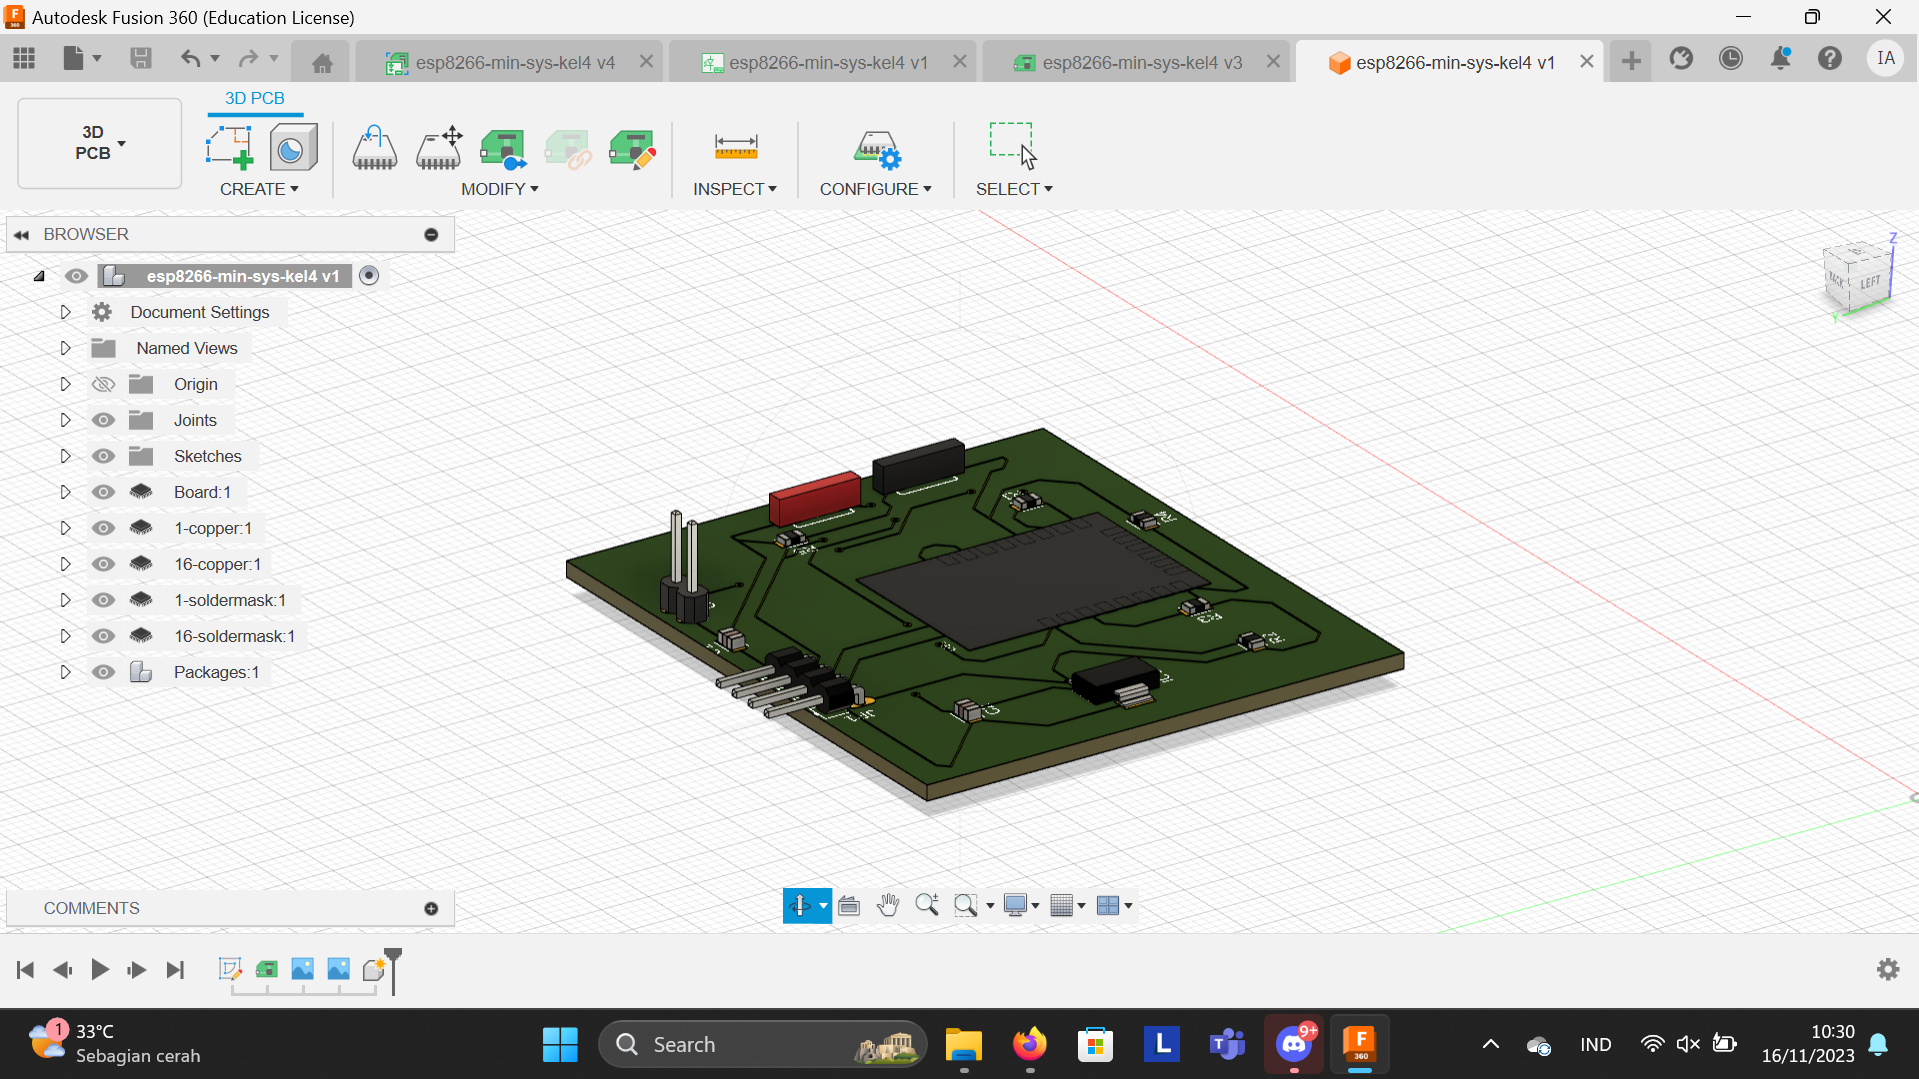
\includegraphics[width=0.4\textwidth]{img/fusion360.png}
    \caption{3D Model dari PCB yang telah dibuat}
    \label{fig:3dmodel}
\end{figure}

Praktikum secara teknis terdapat kendala kecil, seperti :

\begin{enumerate}
    \item Praktikan tidak menggunakan mouse, sehingga proses \textit{design} menjadi lebih lama.
    \item Device yang digunakan untuk praktikum tidak memiliki spesifikasi yang cukup untuk menjalankan Fusion 360, sehingga proses \textit{design} menjadi lebih lama.
\end{enumerate}

% \begin{table}[h]
%     \centering
%     \caption{Caption tabelnya}
%     \label{tab:labelini}
%     \begin{tabular}{|c|c|c|}
%     \hline
%     Kolom 1 & Kolom 2 & Kolom 3 \\
%     \hline
%     Data 1 & Data 2 & Data 3 \\
%     Data 4 & Data 5 & Data 6 \\
%     \hline
%     \end{tabular}
% \end{table}
% Bagian Lampiran
\section*{Lampiran} % Jika ada lampiran

\begin{figure}[H]
  \centering
  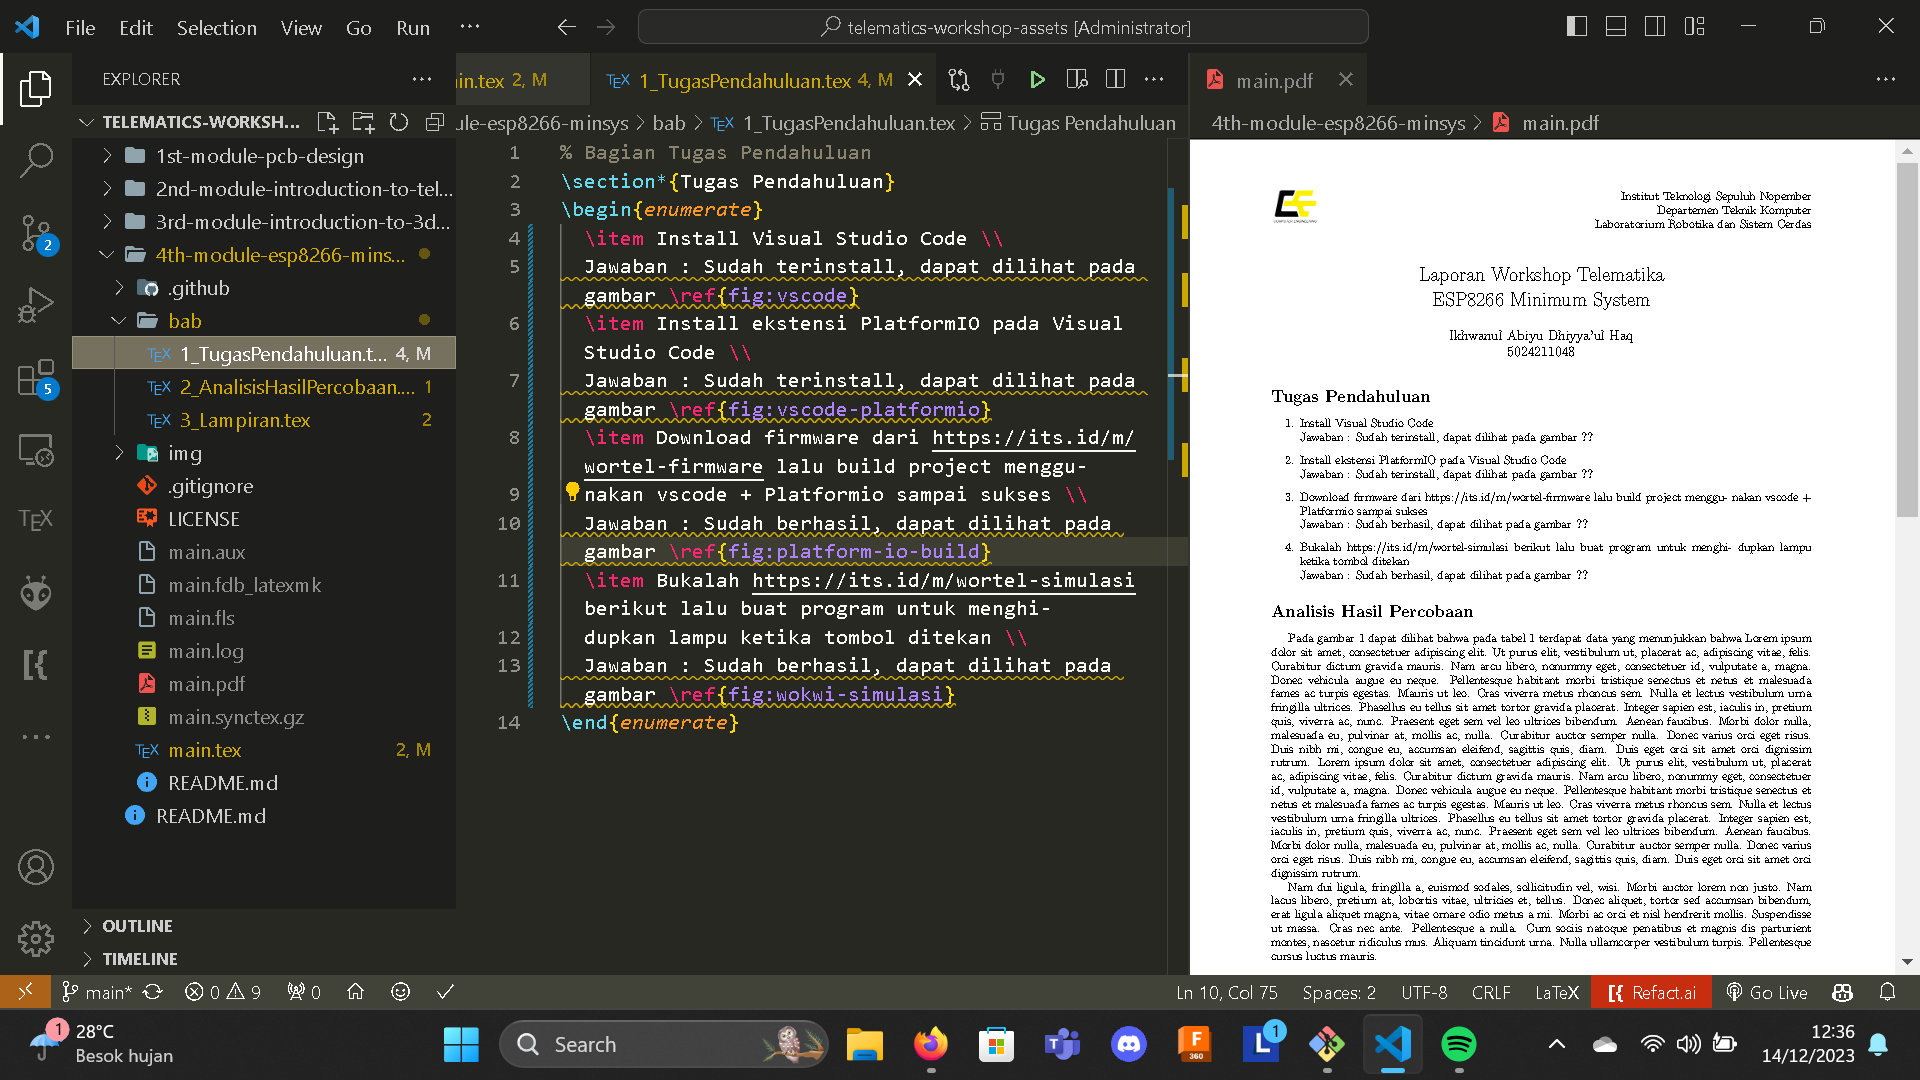
\includegraphics[width=0.8\textwidth]{img/vscode-install.png}
  \caption{Visual Studio Code yang sudah terinstall}
  \label{fig:vscode}
\end{figure}

\begin{figure}[H]
  \centering
  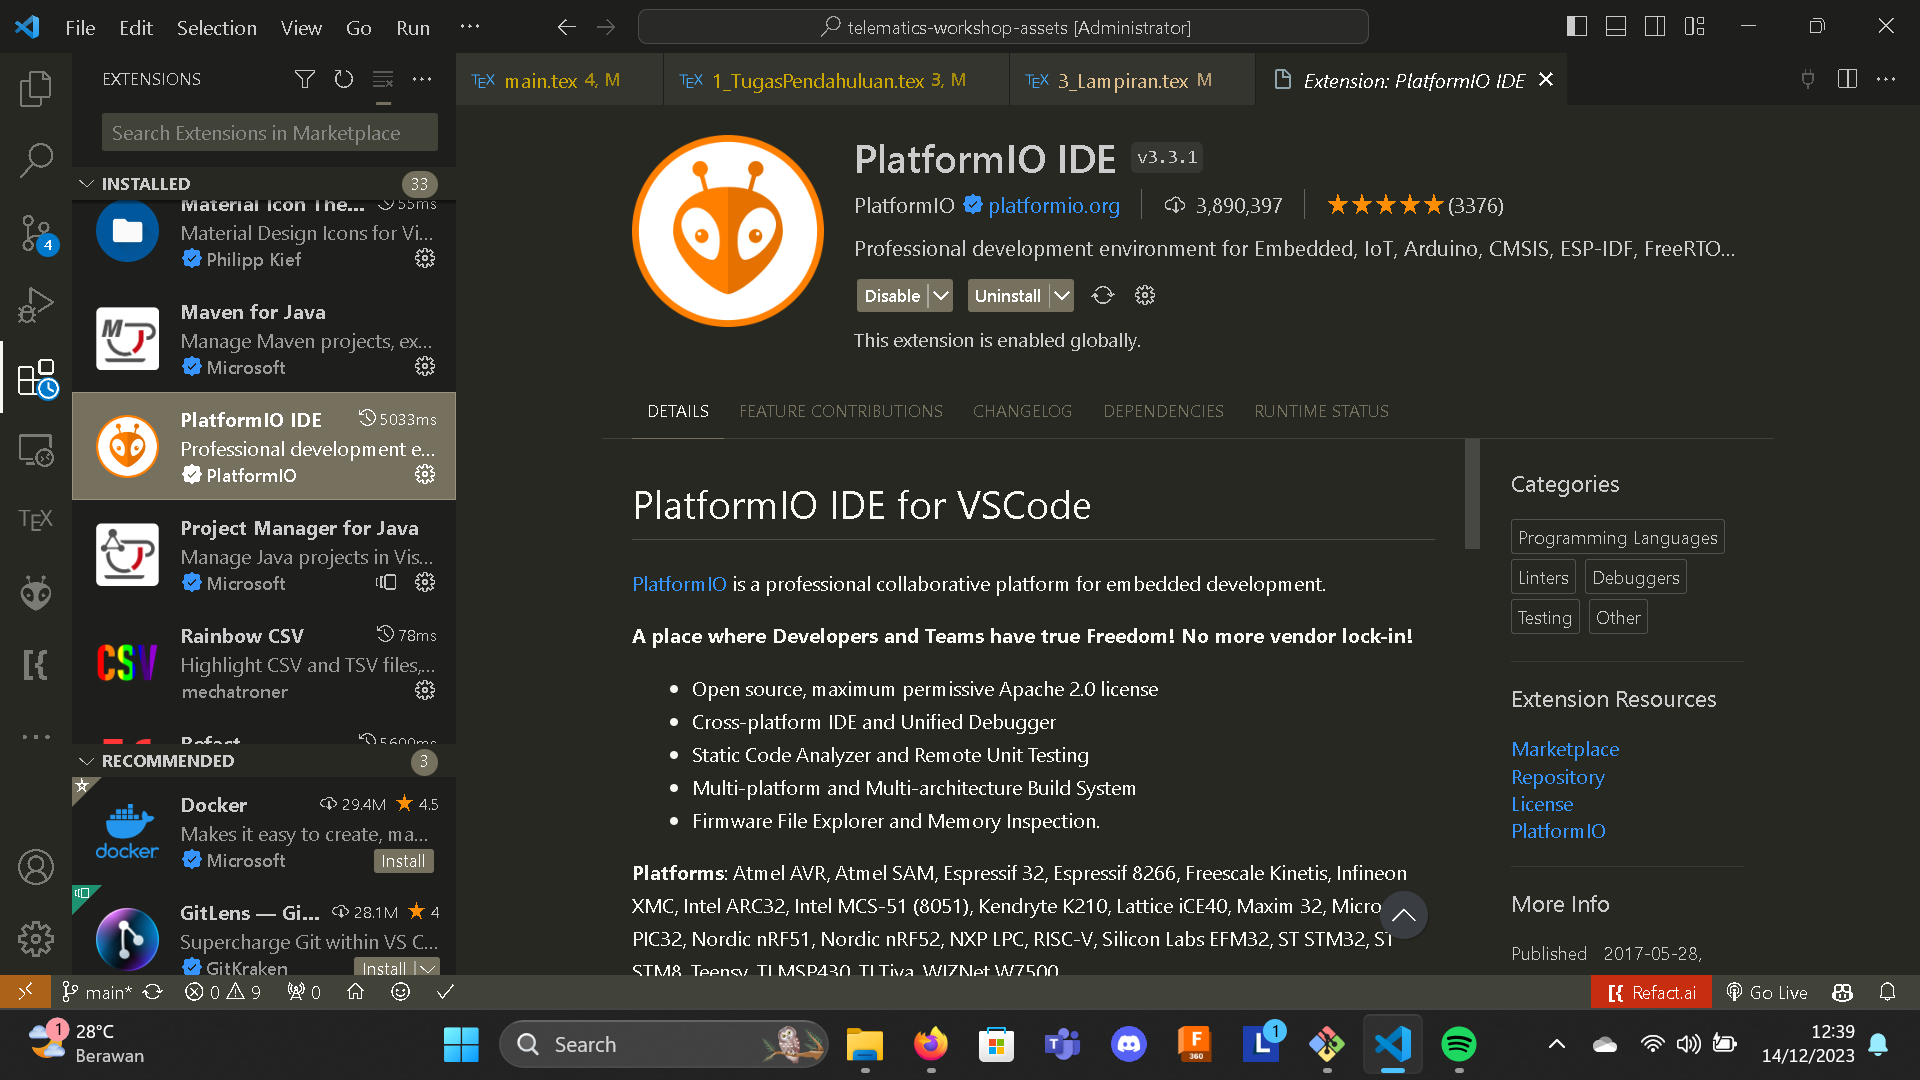
\includegraphics[width=0.8\textwidth]{img/platformio.png}
  \caption{Ekstensi PlatformIO pada Visual Studio Code yang sudah terinstall}
  \label{fig:vscode-platformio}
\end{figure}

\begin{figure}[H]
  \centering
  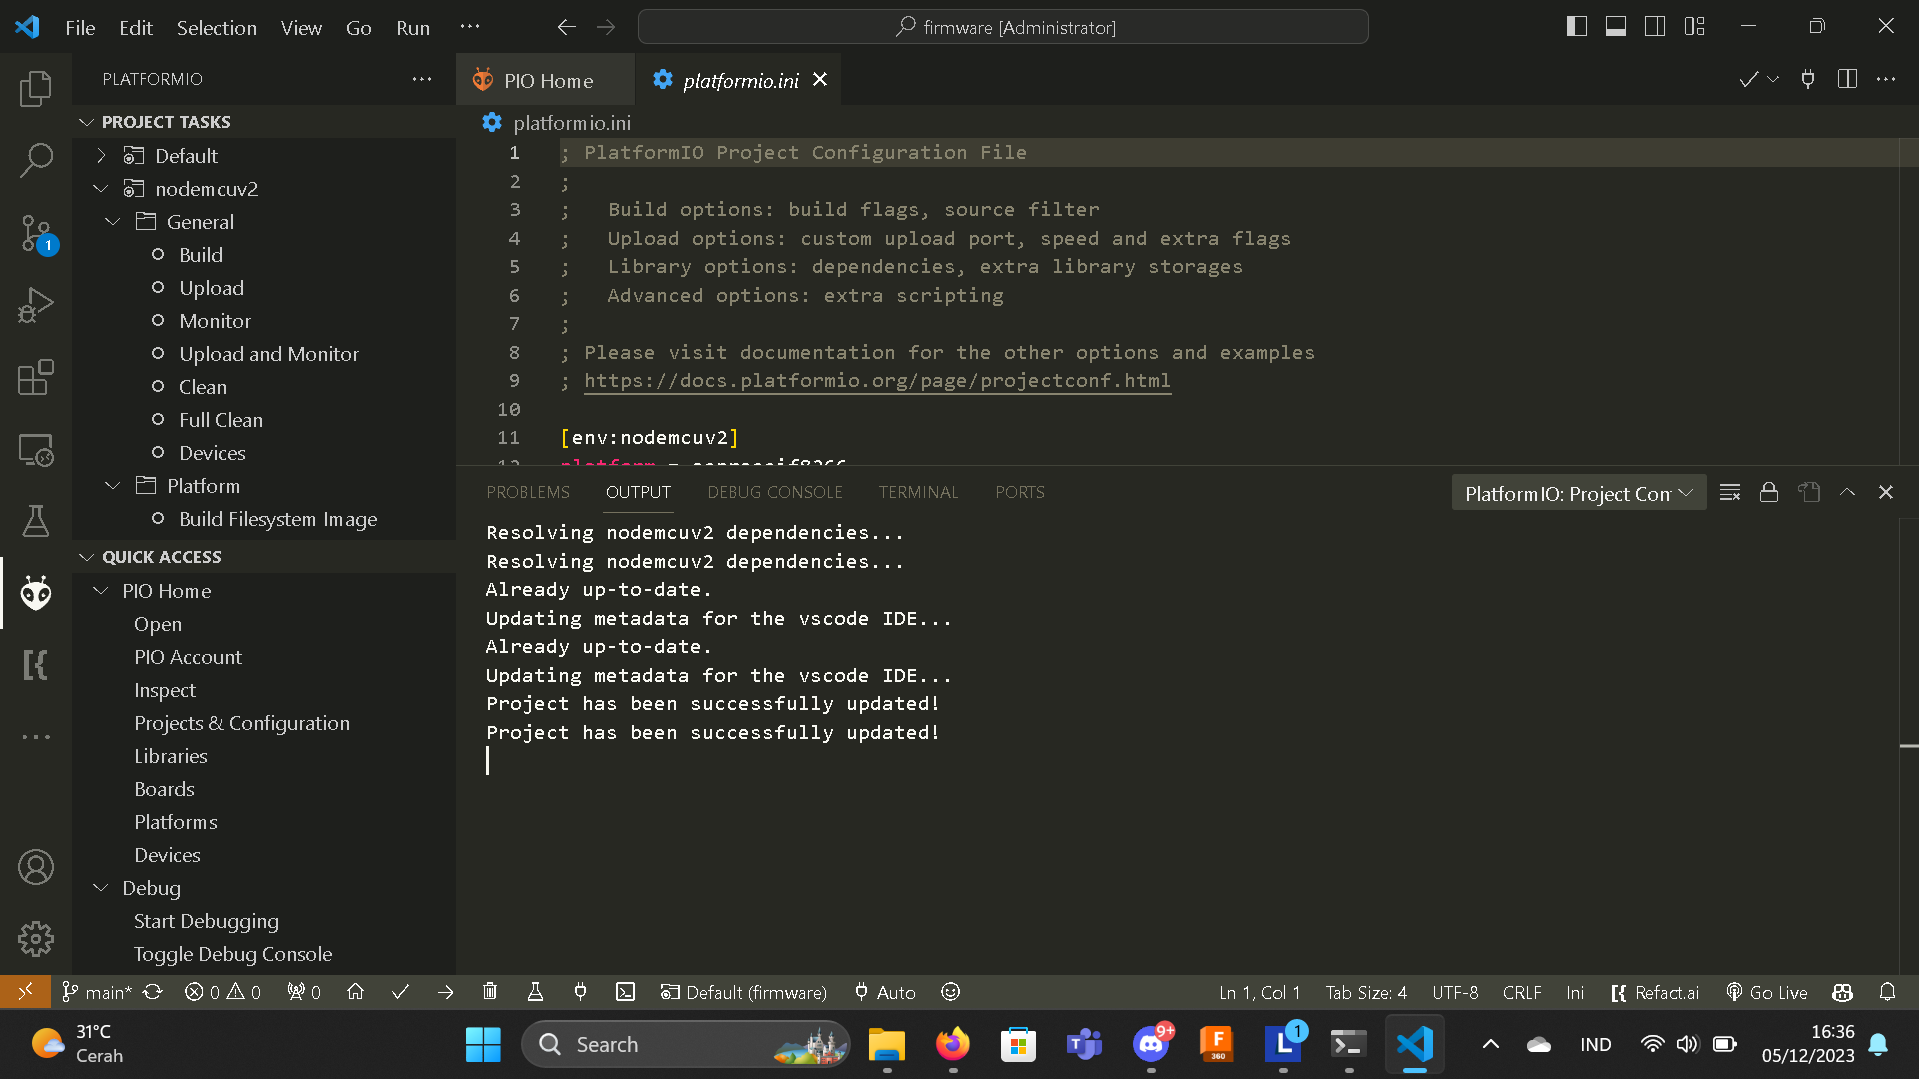
\includegraphics[width=0.8\textwidth]{img/platformio-build.png}
  \caption{PlatformIO berhasil melakukan build}
  \label{fig:platform-io-build}
\end{figure}

\begin{figure}[H]
  \centering
  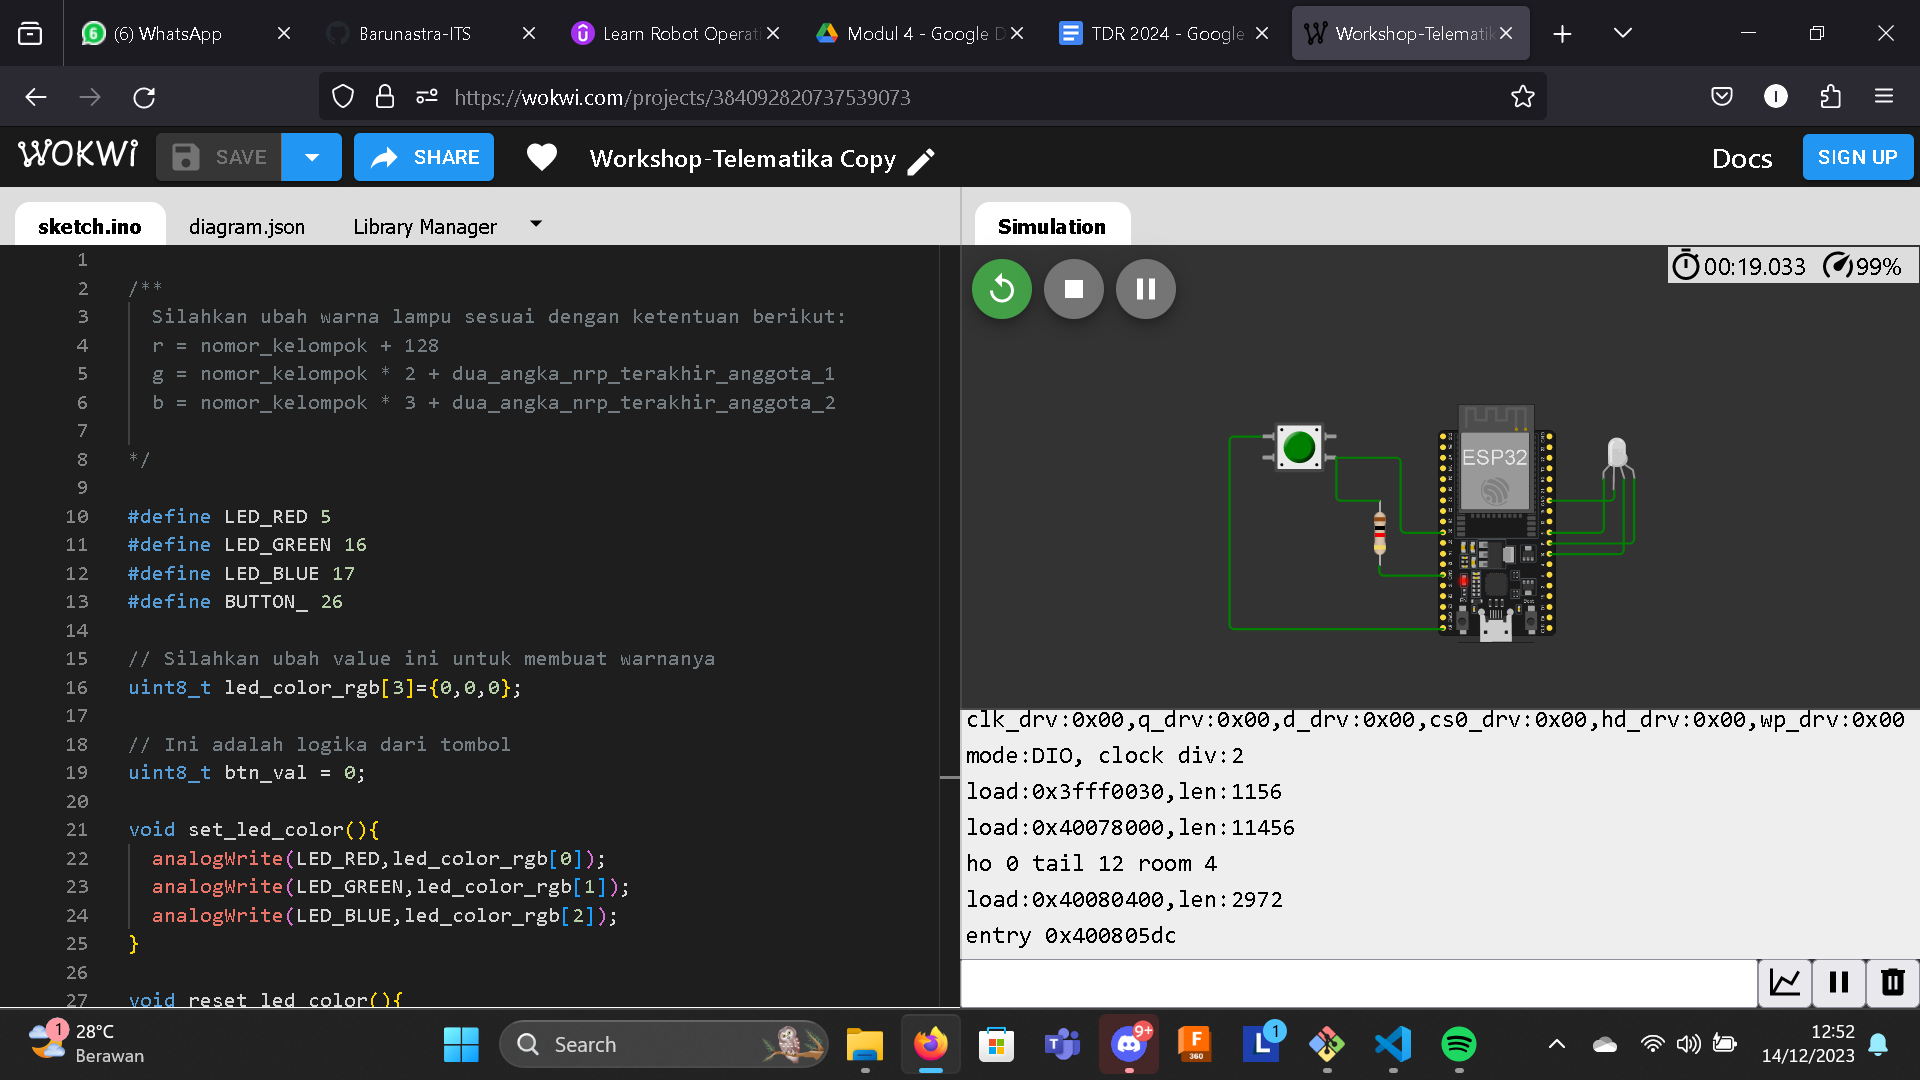
\includegraphics[width=0.8\textwidth]{img/wokwi-simulation.png}
  \caption{Wokwi berhasil melakukan simulasi}
  \label{fig:wokwi-simulasi}
\end{figure}

\begin{figure}[H]
  \centering
  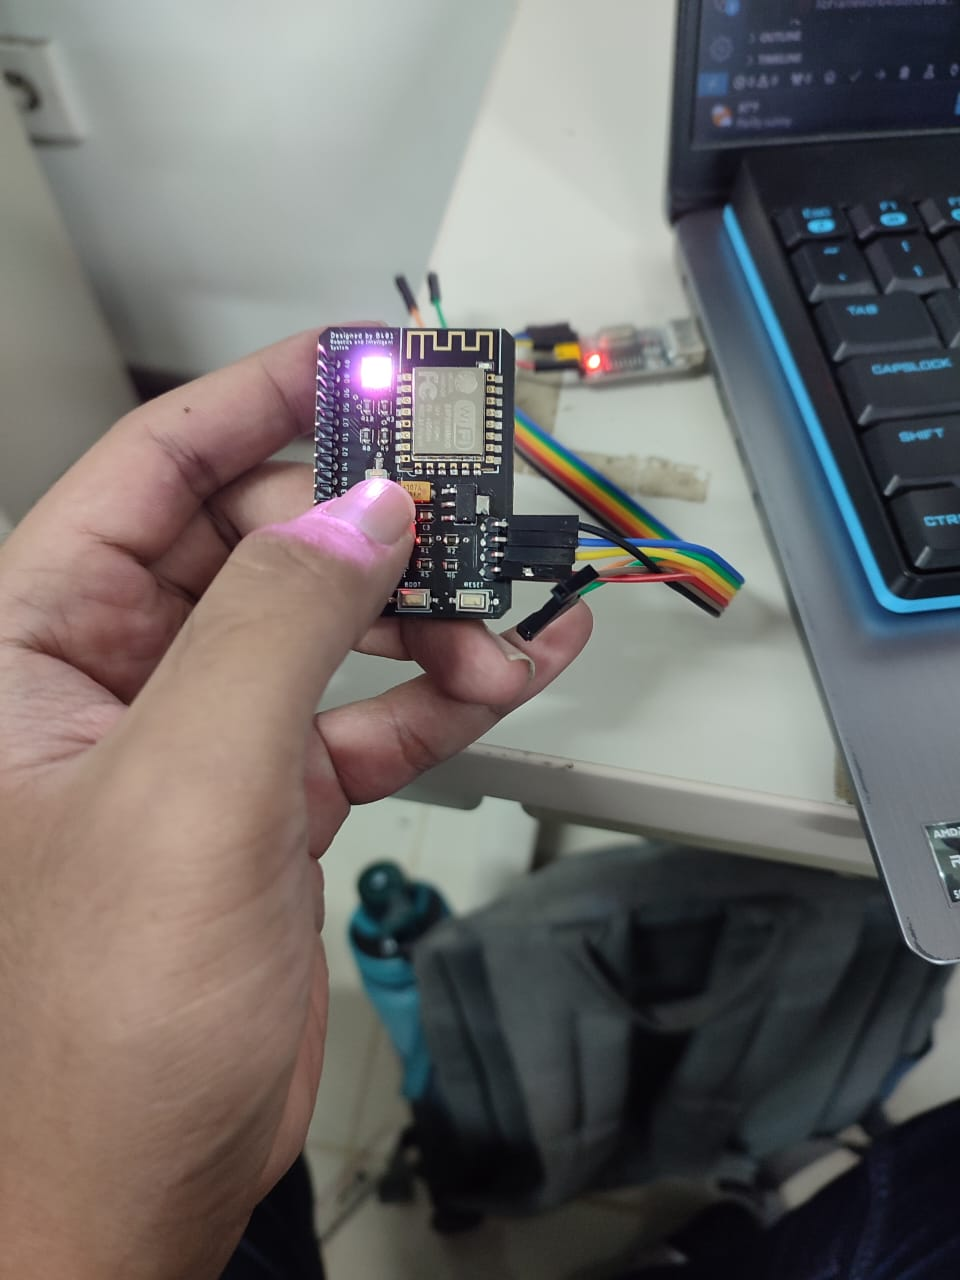
\includegraphics[width=0.8\textwidth]{img/esp-jadi.jpeg}
  \caption{ESP dengan program yang sudah diupload}
  \label{fig:ESP-jadi}
\end{figure}
\end{document}